In questo capitolo verranno descritte nel dettaglio le implementazioni di feature core del Vadalog Reasoner, di cui mi sono occupato durante il mio periodo di Tesi, per l'esecuzione di programmi Vadalog. \newline
Il capitolo è organizzato come segue. Nella sezione 3.1 verranno descritte nel dettaglio le tecniche di ottimizzazione e le loro implementazioni, entreremo nel dettaglio dell'implementazione di ottimizzazioni note come \emph{Push Selections Down} e \emph{Push Projections Down}, ottimizzazioni in presenza di regole composti da più atomi nella testa ed in presenza di join multipli nel corpo di una regola ed infine dei dettagli sulla ricorsione e la loro ottimizzazione. \newline
Nella sezione 3.2 verranno descritte le modalità di esecuzione delle annotazioni post-processing, l'architettura di gestione e l'implementazione delle operazioni dei tipi di dato nel Vadalog Reasoner, la gestione e l'implementazione delle nuove sorgenti ed infine l'implementazione e l'utilizzo delle funzioni e delle query parametriche in Vadalog. \newline
Infine nella sezione 3.3 troveremo una descrizione sull'implementazione dell'editor grafico e della visualizzazione del grafo d'accesso.

\section{Tecniche di ottimizzazione}

Inizialmente il Vadalog Reasoner, effettuava ben poche ottimizzazioni e non permettevano un guadagno sull'esecuzione di programmi, ciò portava ad un limite del Vadalog Reasoner anche in ambito Big Data. \newline
Le tecniche di ottimizzazione sono basate sulla riscrittura, ovvero quando viene lanciato un programma esso viene riscritto applicando le ottimizzazioni ed infine dato in pasto al \emph{Vadalog Reasoner}.
In questa sezione descriveremo le ottimizzazioni di push selections e projections down (sezione 3.1.1), la gestione di teste e join multipli (sezione 3.1.2) e l'individuazione ed inversione delle ricorsioni destre (sezione 3.1.3).

\subsection{Push selections e projections down}

In questa sezione verranno descritte come sono state gestite le operazioni di push selections e projections down all'interno del Vadalog Reasoner. \newline
Queste operazioni rappresentano delle ottimizzazioni note nel settore basi di dati da diversi anni, il loro obiettivo è la trasformazione di una query in un'altra equivalente (stesso risultato), ma anticipando selezioni e proiezioni, in modo da avere dei benefici sui costi temporali e computazionali. \newline
Nel nostro caso, poiché ci troviamo di fronte ad un linguaggio della famiglia Datalog$^\pm$, tali operazioni creano molte problematiche in più rispetto a linguaggi base di interrogazione per database, come SQL. \newline
Questo perché Datalog ha molti più casi da gestire rispetto al linguaggio SQL, ad esempio, vanno gestite le ricorsioni, le variabili esistenziali, regole che possono avere in testa l'atomo A, sul corpo l'atomo B ed un'altra regola che può avere in testa l'atomo B e sul corpo l'atomo A (un ciclo) e quant'altro. \newline \newline
Nella fase di push selections down, l'obiettivo è quello di anticipare le selezioni il prima possibile, ovvero cercare di anticipare le selezioni il più vicino possibile alle regole che coinvolgono nodi di input. Come possiamo vedere nell'esempio~\ref{ex1} (un caso base): 
\begin{example}\label{ex1}
\begin{lstlisting}
	
	b(1). 
	b(2). 
	a(X) :- b(X). 
	d(X) :- a(X), X>10. 
	@output("d").
\end{lstlisting}
\end{example}
Dopo la trasformazione diventa: 
\begin{example}\label{ex2}
	\begin{lstlisting}
	
	b(1). 
	b(2). 
	a(X) :- b(X), X>10. 
	d(X) :- a(X). 
	@output("d").
	\end{lstlisting}
\end{example}
Nell'esempio~\ref{ex2} la selezione è stata anticipata alla regola più vicina al nodo input. \newline
Spesso è necessario che una variabile va anticipata in N regole che coinvolgono (selezionano) tutte la stessa variabile che viene selezionata, come possiamo vedere nell'esempio~\ref{ex3}: 
\begin{example}\label{ex3}
	\begin{lstlisting}
	
	b(1). 
	c(30,33). 
	a1(X) :- b(X). 
	a2(X,Y) :- c(X,Y). 
	d(X) :- a1(X), a2(X,Y), X>1. 
	@output("d").
	\end{lstlisting}
\end{example}
Dopo la trasformazione diventa: 
\begin{example}\label{ex4}
	\begin{lstlisting}
	
	b(1). 
	c(30,33). 
	a1(X) :- b(X), X>1. 
	a2(X,Y) :- c(X,Y), X>1. 
	d(X) :- a1(X), a2(X,Y). 
	@output("d").
	\end{lstlisting}
\end{example}
Nell'esempio~\ref{ex4} la variabile X viene utilizzata in due regole, quindi la selezione viene anticipata in entrambe le regole che coinvolgono tale variabile. \newline
In entrambe le fasi di push selections e projections down, si tiene conto della posizione della variabile nell'atomo anziché del nome della variabile, questo perché in altre regole i nomi delle variabili possono essere in ordine inverso, ne vediamo un'applicazione negli esempi~\ref{ex5} e \ref{ex6}:
\begin{example}\label{ex5}
	\begin{lstlisting}
	
	b1(10,25). 
	c1(25,10). 
	b(Y,X) :- b1(X,Y). 
	c(X,Y) :- c1(X,Y). 
	a(X) :- b(X,Y),c(Y,X),X>20. 
	@output("a").
	\end{lstlisting}
\end{example}
Viene trasformato in:
\begin{example}\label{ex6}
	\begin{lstlisting}
	
	b1(10,25). 
	c1(25,10). 
	b(Y,X) :- b1(X,Y), Y>20. 
	c(X,Y) :- c1(X,Y), Y>20. 
	a(X) :- b(X,Y),c(Y,X). 
	@output("a").
	\end{lstlisting}
\end{example}
Come possiamo vedere nell'esempio~\ref{ex6} la variabile su cui viene effettuata la selezione 'X', che corrisponde alla prima posizione dell'atomo b ed alla seconda posizione dell'atomo c, quando viene anticipata viene opportunamente cambiata di nome in base alla regola. \newline \newline
La fase di push projections down si occupa di anticipare le selezioni il più vicino possibile ai nodi di input ed inoltre di rimuovere le proiezioni inutilizzate, ad esempio se in una regola proietto due variabili, in cui una non è coinvolta con l'output o con un'interazione per produrre l'output. Possiamo vederne un'applicazione nell'esempio~\ref{ex7} e \ref{ex8}:
\begin{example}\label{ex7}
	\begin{lstlisting}
	
	a(2). 
	b(1,1). 
	q(X,Y) :- b(X,Y). 
	c(X) :- a(X), q(X,Y). 
	d(X) :- c(X). 
	@output("d").
	\end{lstlisting}
\end{example}
Che viene trasformato in:
\begin{example}\label{ex8}
	\begin{lstlisting}
	
	a(2). 
	b(1,1). 
	q(X,Y) :- b(X,Y). 
	c(X) :- a(X), q(X). 
	d(X) :- c(X). 
	@output("d").
	\end{lstlisting}
\end{example}
Come possiamo vedere nell'esempio~\ref{ex8}, nella regola c(X) :- a(X), q(X,Y) viene eliminata la variabile 'Y' poiché inutilizzata. \newline
Mentre l'applicazione della proiezione anticipata, possiamo vederla nell'esempio~\ref{ex9} e \ref{ex10}:
\begin{example}\label{ex9}
	\begin{lstlisting}
	
	b(1). 
	c(2,5). 
	a1(X) :- b(X). 
	a2(X,Y) :- c(X,Y). 
	d(X) :- a1(X), a2(X,5). 
	@output("d").
	\end{lstlisting}
\end{example}
Che viene trasformato in:
\begin{example}\label{ex10}
	\begin{lstlisting}
	
	b(1). 
	c(2,5). 
	a1(X) :- b(X). 
	a2(X) :- c(X,5). 
	d(X) :- a1(X), a2(X). 
	@output("d").
	\end{lstlisting}
\end{example}
Nell'esempio~\ref{ex10} viene anticipata la proiezione dell'atomo 'c', e viene rimossa la variabile 'Y' dall'atomo 'a2', poiché inutilizzata. \newline \newline
L'implementazione delle procedure di push selections e projections down è stata effettuata come una riscrittura del programma, ovvero prima di mandare il codice in pasto al reasoner, esso viene opportunamente trasformato seguendo le tipologie di ottimizzazioni sopra descritte. \newline
Nella fase di push selections down, si visita il grafo d'esecuzione partendo dai nodi di output, durante la quale vengono controllate tutte le variabili delle condizioni della regola corrente, e si fa un match con le variabili degli atomi nel corpo della regola, a questo punto ci sono due possibili strade da percorrere: 
\begin{itemize}
	\item La variabile occorre in N atomi nel corpo e tutti gli atomi sono di input. In questo caso la condizione viene lasciata nella regola corrente, poiché non è possibile anticipare la selezione, si continua poi la visita del grafo per vedere se ci sono altre selezioni che è possibile anticipare.
	\item La variabile occorre in atomi che sono di input e in atomi che non sono di input. In questo caso, viene lasciata la condizione alla regola corrente, ma si tiene conto degli altri atomi (che non sono di input) coinvolti, proseguendo la visita del grafo, quando arriveremo alle regole che hanno tali atomi in testa, vengono nuovamente verificati gli atomi nel corpo, nel caso in cui siano tutti di input allora viene aggiunta la selezione anche a queste regole, altrimenti si prosegue finché non arriviamo alla regola contenente soltanto atomi di input.
\end{itemize}
La fase di push projections down è molto simile, ma anziché controllare le condizioni, in ogni regola si verifica la presenza di costanti, in caso positivo si procede con lo stesso criterio del push selections down. Inoltre si verifica anche la presenza di variabili inutili, ad esempio nella testa ho le variabili [X,Y] e nel corpo [X,Y,J], in questa caso, J viene rimossa dall'atomo nel corpo della regola e conseguentemente dalla testa della regola contenente l'atomo coinvolto.

\subsection{Gestione di teste multiple e join multipli}

In questa sezione verranno descritte le ottimizzazioni in presenza di teste e join multipli. \newline
Vadalog è un linguaggio che permette regole standard da poter utilizzare nella forma head :- body, dove head è rappresentato da un singolo atomo e body da una lista di atomi e una lista di condizioni. \newline
Tuttavia, vogliamo gestire diverse funzionalità che permettono un'espressività maggiore, una di queste è la possibilità di definire una regola con più teste, ad esempio se ho diversi atomi che sono composti dallo stesso corpo anziché far scrivere al programmatore un numero di regole pari al numero di atomi, viene effettuata una riscrittura che permette di scrivere una regola con più teste, possiamo vederne un'applicazione nell'esempio~\ref{ex11}. 
\begin{example}\label{ex11}
	\begin{lstlisting}
	
	h1(X,Y),h2(Y,Z),h3(Z,W) :- a(X,Y,Z),b(Z,M).
	\end{lstlisting}
\end{example}
Dove gli atomi h1, h2, h3 condividono lo stesso corpo. \newline
In questo caso viene riscritto, prima di essere dato in pasto al Vadalog Reasoner come nell'esempio~\ref{ex12}: 
\begin{example}\label{ex12}
	\begin{lstlisting}
	
	h_tmp(X,Y,Z,M) :- a(X,Y,Z),b(Z,M). 
	h1(X,Y) :- h_tmp(X,Y,Z,M). 
	h2(Y,Z) :- h_tmp(X,Y,Z,M). 
	h3(Z,W) :- h_tmp(X,Y,Z,M). 
	\end{lstlisting}
\end{example}
Viene quindi definita una regola standard che contiene il corpo condiviso con le N teste, e aggiunta una regola lineare (uno ed un solo atomo nel corpo) per ogni testa. \newline
Inoltre è anche possibile definire delle regole "speciali", che hanno una sintassi diversa da quelle standard. Tali regole coinvolgono la testa della regola, permettendo di utilizzare un'uguaglianza come testa. \newline
Tali regole vengono tradotte in regole esistenziali e implicitamente trattate come regole di output. Vediamo la trasformazione negli esempi~\ref{ex17} e \ref{ex18}:
\begin{example}\label{ex17}
	\begin{lstlisting}
	
		Y=Z :- a(X,Y),a(X,Z).
	\end{lstlisting}
\end{example}
Che viene trasformato in: 
\begin{example}\label{ex18}
	\begin{lstlisting}
	
	egd1(X,Y,Z,J) :- a(X,Y),a(X,Z),J=Y==Z.
	@output("egd1").
	\end{lstlisting}
\end{example}
Viene quindi creato un apposito atomo di testa che chiameremo \emph{$egd_{N}$} ed una variabile esistenziale \{$J_{1}$, $J_{2}$, ..., $J_{n}$\}. L'atomo in testa proietta tutte le variabili del corpo (compresa la variabile esistenziale) ed aggiunge come condizione l'assegnazione della variabile esistenziale, che sarà quella espressa in testa ed infine viene aggiunta la regola di output per ogni atomo $egd_{N}$. Anche questa funzionalità è stata implementata utilizzando una riscrittura prima della procedura di reasoning. \newline \newline
Spesso sono presenti regole, che nel corpo hanno più di 2 atomi che sono vincolati tramite l'operazione di join, l'uno con l'altro (ad esempio join tra tre elementi o join incrociati tra tre atomi). \newline
Quando sono presenti join tra tre o più atomi, l'aumento del tempo di computazione è proporzionale alla crescita del numero di atomi interessati. Vediamo un'applicazione pratica nell'esempio~\ref{ex13}:
\begin{example}\label{ex13}
	\begin{lstlisting}
	
	c(Z,X,M) :- a(X,Y),b(Y,K),c(K,M).
	\end{lstlisting}
\end{example}
Nell'esempio~\ref{ex13} gli atomi a, b e c sono coinvolti in un join incrociato, ovvero l'atomo a è in join con b e quest'ultimo con c. \newline
Nella riscrittura la regola generalizzata composta da N atomi, di cui M (>=3) sono in join tra loro, viene splittata in M regole in cui vengono definiti join tra due elementi soltanto, e gli atomi non coinvolti nel join, vengono inseriti nella regola finale. \newline
Nell'esempio~\ref{ex14} è possibile vedere il programma dopo il processo di riscrittura: 
\begin{example}\label{ex14}
	\begin{lstlisting}
	
	v_atom1(X,K) :- a(X,Y),b(Y,K). 
	c(Z,X,M) :- v_atom1(X,K),c(K,M).
	\end{lstlisting}
\end{example}
Il join viene quindi splittato in due regole, dando il medesimo risultato di output.

\subsection{Individuazione e inversione delle ricorsioni destre}

Un altro collo di bottiglia per il tempo di computazione e l'efficienza è la ricorsione, in particolare le ricorsioni destre (atomo che ricorre si trova alla fine del corpo della regola) risultano meno efficienti delle ricorsioni sinistre (atomo che ricorre si trova all'inizio del corpo della regola). \newline
Tale perdita di efficienza si ha sopratutto in presenza di join. Ricordiamo che Vadalog utilizza un algoritmo di join simile al nested loop (ogni ennupla della prima relazione viene paragonata ad ogni ennupla della seconda relazione). \newline
Supponiamo che ci sia una regola Vadalog del tipo head :- A,B, dove A è un atomo non ricorsivo e B un atomo ricorsivo, quindi una ricorsione destra, e che A abbia N ennuple, e B abbia M ennuple. \newline
Quando andiamo ad effettuare il nested loop join, ogni ennupla di A effettua una chiamata ricorsiva su B (per paragonarla) per tutte le ennuple di B, vengono quindi fatte NxM chiamate ricorsive circa. \newline
Nel caso in cui la regola abbia una ricorsione sinistra (quindi dopo la riscrittura), ovvero head :- B,A, in  questo caso è B che viene paragonata ad A, quindi vengono prima fatte le chiamate ricorsive e poi il risultato delle chiamate paragonato alle ennuple di B, quindi vengono fatte M chiamate ricorsive circa. Quindi la riscrittura porta un guadagno notevole sulla base del numero di chiamate ricorsive. \newline
Vediamo un'applicazione pratica di come avviene la riscrittura negli esempi~\ref{ex15} e \ref{ex16}: 
\begin{example}\label{ex15}
	\begin{lstlisting}
	
	a(Y) :- b(X,Y), a(X).
	\end{lstlisting}
\end{example}
Viene trasformato in:
\begin{example}\label{ex16}
	\begin{lstlisting}
	
	a(Y) :- a(X), b(X,Y).
	\end{lstlisting}
\end{example}
L'algoritmo di riscrittura ha lo scopo di portare l'atomo ricorsivo come primo atomo del corpo, il resto della regola rimane invariato, come il risultato finale.

\section{Supporto a nuovi tipi di dato, sorgenti e funzionalità}

Nel linguaggio Vadalog vengono supportati: diversi tipi di dato, semplici e strutturati; diverse sorgenti dati da cui prendere gli input, ad esempio da un database; diverse funzionalità varie che garantiscono l'usabilità all'utente finale: ad esempio la possibilità di fare operazioni standard dopo il calcolo del risultato (orderby, distinct, ecc.), possibilità di definire funzioni e query parametriche. \newline
In seguito verranno descritte nel dettaglio le annotazioni post-processing (sezione 3.2.1), l'architettura utilizzata per la gestione dei tipi di dato e le loro operazioni con relativa implementazione (sezione 3.2.2) ed infine la gestione e l'utilizzo di funzioni e query parametriche in Vadalog (sezione 3.2.3).

\subsection{Post-processing annotations}

Le post-processing annotations sono delle annotazioni speciali in Vadalog che permettono di effettuare dei calcoli dopo tutta la procedura di reasoning. 
In queste annotazioni è possibile specificare molte operazioni che si possono effettuare:
\begin{itemize}
	\item \emph{Order by}: ha l'obiettivo di ordinare l'output per un determinato atomo, specificandone il campo (variabile) sul quale ordinare.
	\item \emph{Min}: calcola il valore minimo per una o più posizioni in un atomo e raggruppa per le altre. Ad esempio se viene definito il minimo sul terzo campo ed ho come risultato: a(1,"a",1), a(1,"a", 5) ed a(1,"b",3), il risultato finale sarà a(1,"a",1) e  a(1,"b",3).
	\item \emph{Max}: ha lo stesso comportamento di Min, ma prendendo il massimo.
	\item \emph{Argmin}: ha la stessa funzionalità di Min, soltanto che è possibile definire le posizioni su cui raggruppare anziché prenderle tutte di default. 
	\item \emph{Argmax}: stesso comportamento di Argmin, ma con il massimo.
	\item \emph{Unique}: ha la funzionalità di rimuovere i duplicati dall'output di un atomo definito.
	\item \emph{Certain}: si occupa di rimuovere, dall'output di un atomo definito, i fatti che contengono nulli. Utile quando si devono effettuare salvataggi su database.
\end{itemize}
Io mi sono occupato dell'implementazione delle operazioni di Argmin ed Argmax. \newline
Negli esempi~\ref{ex19} e \ref{ex20} vediamo l'applicazione di Argmax e il risultato ottenuto.
\begin{example}\label{ex19}
	\begin{lstlisting}
		
	f(1,3,"a",3).
	f(4,3,"a",5).
	f(2,6,"b",7).
	f(2,6,"b",8).
	f(3,6,"b",9).
	g(X,Y,Z,K) :- f(X,Y,Z,K).
	@output("g").
	@post("g","argmax(4,<2,3>)").
	\end{lstlisting}
\end{example}
\begin{example}\label{ex20}
	\begin{lstlisting}
	
	g(4,3,"a",5).
	g(3,6,"b",9).
	\end{lstlisting}
\end{example}
Nell'implementazione vengono prima effettuati i raggruppamenti per le posizioni indicate nell'annotazione, e viene poi effettuata la selezione del massimo (o minimo, a seconda dell'annotazione). 

\subsection{Tipi di dato e sorgenti dati}

Vadalog supporta molti tipi di dato semplici e strutturati, di conseguenza supporta le operazioni che possono essere effettuate su questi tipi di dato. Sono presenti diversi tipi di dato in Vadalog: \emph{integer}, \emph{double}, \emph{string}, \emph{boolean}, \emph{date}, \emph{set} e \emph{Marked Null}. \newline
Nel Vadalog Reasoner la gestione dei tipi di dato e le eventuali operazioni viene effettuata utilizzando il pattern architetturale \emph{Visitor}, che permette di separare un algoritmo dalla struttura di oggetti composti a cui è applicato, in modo da poter aggiungere nuove operazioni e comportamenti senza dover modificare la struttura stessa~\cite{gamma1995design}. È presente una classe che si occupa di eseguire le operazioni che è chiamata \emph{Visitor} e diverse classi chiamate \emph{ConcreteElement} che estendono la classe \emph{Element}. Il Visitor implementa un metodo "visit" per ogni classe concreta (riconoscerà quale invocare basandosi sulla classe del chiamante) e le varie classi concrete implementano un metodo "accept" che invoca "visit" passando se stesso come parametro per permettere di accedere al proprio stato. \newline
Nel Vadalog Reasoner il \emph{Visitor} è chiamato \emph{ExpressionVisitor}, e le \emph{ConcreteElement}, rappresentano tutte le espressioni che possono essere applicate ai tipi di dato. Nella Figura~\ref{fig:visitoruml} possiamo vedere una porzione del diagramma delle classi riguardante l'applicazione del pattern architetturale. 
\begin{figure}[h]
	\centering
	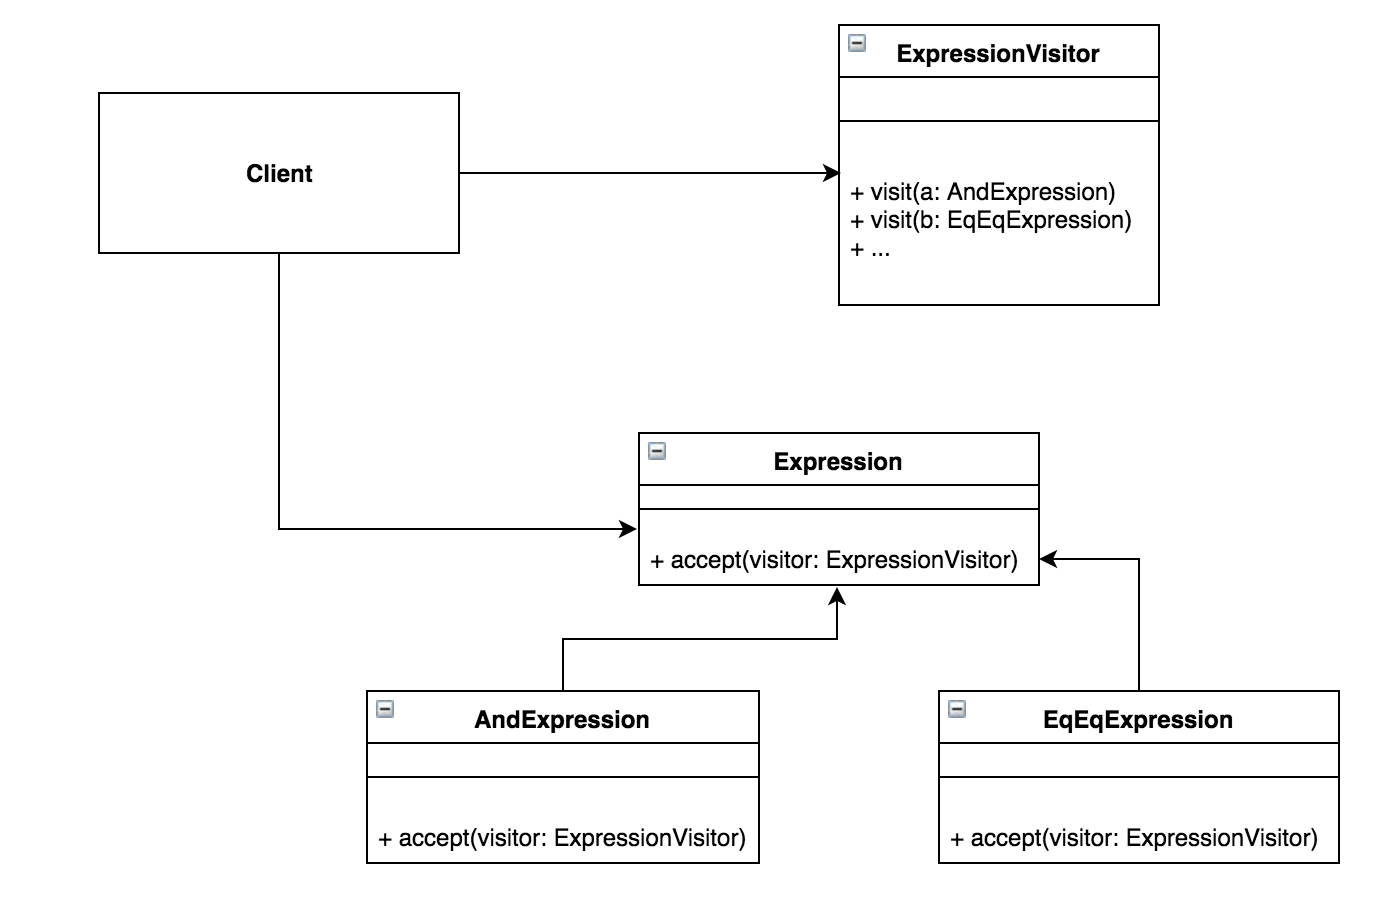
\includegraphics[width=0.8\linewidth]{figure/visitor_uml}
	\caption{Diagramma delle classi del pattern Visitor.}
	\label{fig:visitoruml}
\end{figure}

Il client invoca i metodi di accept e conseguentemente l'ExpressionVisitor che esegue le operazioni a seconda del chiamante. \newline
Io mi sono occupato dell'integrazione completa (tipi e operazioni base) dei tipi boolean e date con l'integrazione delle operazioni base per le stringhe, dove ogni operazione rappresentava un metodo nell'Expression Visitor. \newline
Per il tipo semplice \emph{boolean} ho definito le operazioni di AND, OR, NOT, ==, <>, >, <, >= e <= utilizzando i confronti forniti da Java. Mentre per il tipo strutturato \emph{date}, come prima operazione mi sono occupato del cast dal tipo utilizzato in Vadalog (YYYY-MM-DD HH24:MI:SS) al tipo Java (GregorianCalendar) ed in seguito delle operazioni di confronto ==, <>, >, <, >= e <=. Infine mi sono occupato dell'implementazione degli operatori per le stringhe in Vadalog: substring, contains, strartsWith, endsWith, concat ed indexOf, utilizzando anche qui le primitive Java.  \newline \newline
Vadalog inoltre supporta diverse sorgenti dati come input, al momento sono presenti le seguenti sorgenti:
\begin{itemize}
	\item \emph{File CSV locali}: lettura e scrittura di dati in file CSV salvati su disco fisso.
	\item \emph{File CSV remoti}: download e lettura di dati in file CSV in internet, con l'utilizzo del protocollo HTTP.
	\item \emph{Postgres}: lettura e scrittura di dati su database Postgres.
	\item \emph{OXPath}: lettura di dati provenienti da pagine html sul web.
\end{itemize}
Nel Vadalog Reasoner per l'implementazione e la gestione delle sorgenti dati si è fatto uso di polimorfismo, è presente una classe \emph{RecordManager}, che viene estesa da classi concrete che rappresentano le possibili sorgenti. \newline
In Figura~\ref{fig:recordmanageruml} possiamo vedere un diagramma delle classi che rappresenta la gestione del record manager e le varie classi concrete nel Vadalog Reasoner. \newline
Io mi sono occupato dell'integrazione di file CSV sia remoti che locali. Poiché le implementazioni sono molto simili, l'unica differenza sostanziale è la lettura del file, una avviene in locale ed una bisognava effettuare il download del file, ho quindi deciso di introdurre un'ulteriore forma di polimorfismo creando una classe astratta \emph{CSVRecordManager} che implementa tutte le operazioni in comune, estesa da due sottoclassi la cui unica funzione è leggere il file. \newline
\begin{figure}[h]
	\centering
	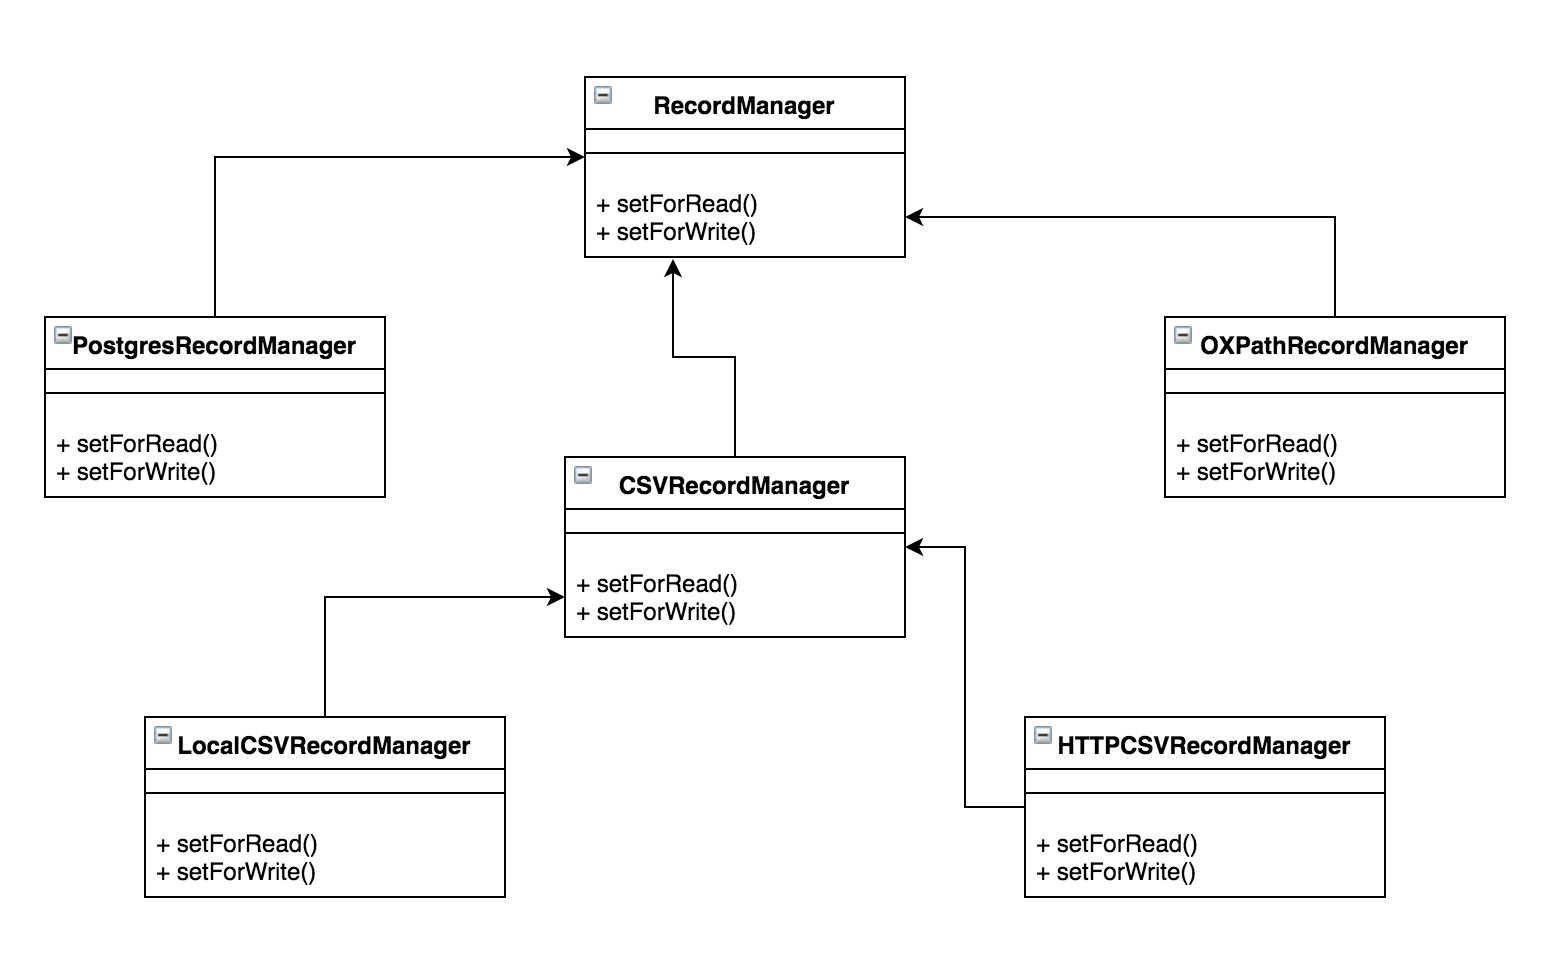
\includegraphics[width=0.8\linewidth]{figure/recordmanageruml}
	\caption{Diagramma delle classi che rappresenta la gerarchia del record manager.}
	\label{fig:recordmanageruml}
\end{figure}

Per l'implementazione di lettura vengono lette le righe del file CSV, successivamente caricate come fatti di input per l'atomo associato. La particolarità è che viene effettuata un'inferenza dei tipi di dato del file CSV attraverso una cascata di \emph{Try/Catch} che tentano di fare il cast del valore. \newline
Per l'implementazione di scrittura viene semplicemente creato un file CSV nel path definito dall'utente e salvato l'output al suo interno.

\subsection{Funzioni e query parametriche}

Vadalog supporta le funzioni (chiamate \emph{funzioni di skolem}), che possono essere implementate con procedure esterne (\emph{user-defined functions}) scritte in altri linguaggi (Java o Python), se non vengono implementate allora producono un nullo. Io mi sono occupato sia dell'integrazione delle funzioni che dell'utilizzo di procedure esterne. \newline
Negli esempi~\ref{ex21} e \ref{ex22} possiamo vedere due utilizzi di funzioni, nell'esempio~\ref{ex21} non è presente nessuna implementazione, viceversa nell'esempio~\ref{ex22}. 
\begin{example}\label{ex21}
	\begin{lstlisting}
	
		b(1,2).
		a(X,Y,Z) :- b(X,Y),Z=#f(X,Y).
		c(K) :- b(X,Y),K=#f(X,Y).
		d(K) :- b(X,Y),K=#g(X,Y).
		@output("a").
		@output("c").
		@output("d").
	\end{lstlisting}
\end{example}\label{ex22}
\begin{example}
	\begin{lstlisting}
	
		b(1,2).
		c(3,2).
		a(Y,Z) :- b(X1,Z),c(X2,Z),Y=#f(X1,X2).
		@output("a").
		@implement("#f","python","com.module1.module2","functionName").
	\end{lstlisting}
\end{example}
Se le funzioni non vengono implementate allora esse producono un nullo, la particolarità è che tale nullo dovrà essere uguale nel caso in cui la stessa funzione prende gli stessi input, ad esempio se nella sostituzione ho la funzione \#f(1,2) e ritorna un valore nullo $Z_{1}$, allora se in un successivo passaggio viene invocata nuovamente la stessa funzione, dovrà restituire lo stesso risultato. \newline
Per implementare questa particolarità ho fatto uso di una cache creata all'inizio del processo di reasoning e distrutta al termine, la quale conteneva i risultati parziali di ogni funzione. \newline
Le funzioni vengono gestite attraverso il Visitor, che ha diversi compiti: 
\begin{itemize}
	\item verifica se la funzione è già stata invocata, in caso positivo restituisce il valore nullo associato alla funzione, altrimenti
	\item verifica se la funzione non ha implementazioni associate, in questo caso genera un nuovo nullo e lo aggiunge in cache, altrimenti
	\item se è stato implementato con una procedura Java, allora importa e con la riflessione invoca il metodo esterno con i parametri passati alla funzione Vadalog, altrimenti
	\item se è stato implementato con una procedura Python, attraverso un tool di Java interpreta ed esegue il codice Python con i parametri passati alla funzione Vadalog.
	\item Infine salva il risultato nella pila di output, ed aggiunge il risultato della funzione in cache.
\end{itemize}
Questa procedura viene eseguita ogni volta che viene utilizzata una funzione nel programma Vadalog. \newline \newline
Mi sono anche occupato dell'implementazione di query parametriche in Vadalog, come già detto è possibile avere diverse sorgenti, in particolare su database relazionali è possibile fare anche delle query per prenderne i risultati con l'annotazione di qbind, come mostrato nell'esempio~\ref{ex23}.
\begin{example}\label{ex23}
	\begin{lstlisting}
		
		test("marco","luigi").
		test("fabio", "antonio").
		control(X,Y) :- own(X,Y,W), W>0.5.
		control(X,Z) :- control(X,Y), own(Y,Z,W), V=msum(<Z>,W), V>0.5.
		@output("control").
		@input("own").
		@bind("own","postgres","vada","ownerships").
		@qbind("own","postgres","vada",
		"select name1, name2, weight 
		from ownerships2
		where name1='Marco'
		").
	\end{lstlisting}
\end{example}
Le query parametriche permettono di utilizzare dei parametri nelle selezioni, come possiamo vedere nell'esempio~\ref{ex24}.
\begin{example}\label{ex24}
	\begin{lstlisting}
	
	test("marco","luigi").
	test("fabio", "antonio").
	control(X,Y) :- own(X,Y,W), W>0.5.
	control(X,Z) :- test(X,Y), own(Y,Z,W), V=msum(<Z>,W), V>0.5.
	@output("control").
	@input("own").
	@bind("own","postgres","vada","ownerships").
	@qbind("own","postgres","vada",
	"select name1, name2, weight 
	from ownerships2
	where name1=\${1}
	").
	\end{lstlisting}
\end{example}
Nelle query parametriche viene specificato un valore del tipo \${1}, che sta a rappresentare i valori in prima posizione dell'atomo corrente. Solitamente il parametro che viene espresso è messo in join con un altro atomo, come avviene nell'esempio~\ref{ex24}, che viene messo in join con "control". In questo caso i valori di \${1} sono "luigi" ed "antonio", vengono quindi effettuate due query una con name1 uguale a "luigi" ed una "antonio". \newline
Spesso invece i valori da sostituire possono essere presi direttamente dai fatti, come possiamo vedere nell'esempio~\ref{ex25}.
\begin{example}\label{ex25}
	\begin{lstlisting}
	
	own("marco",1,2).
	own("luigi",2,3).
	control(X,Y) :- own(X,Y,W), W>0.5.
	@output("control").
	@input("own").
	@bind("own","postgres","vada","ownerships").
	@qbind("own","postgres","vada",
	"select name1, name2, weight 
	from ownerships2
	where name1=\${1}
	").
	\end{lstlisting}
\end{example}
In questo caso vengono effettuate due query, una con name1 uguale a "marco" ed una "luigi". \newline
Per applicare le query parametriche è necessario però garantire la proprietà di \emph{safety}, ovvero che l'atomo p deve avere il parametro che è coinvolto nella qbind in una posizione che non sia dangerous, cioè non deve avere nulli, anche negli altri atomi del corpo. \newline
L'implementazione delle query parametriche è svolta a runtime, in particolare durante il processo di reasoning. L'atomo coinvolto nel qbind viene sempre spostato come ultimo atomo del corpo della regola. Per l'esecuzione di una query parametrica si svolgono le seguenti operazioni: 
\begin{itemize}
	\item Si scorre il grafo di esecuzione eseguendo prima il sottoalbero sinistro, dove vengono visitati tutti gli atomi e raccolti i fatti provenienti da essi e salvati in una cache.
	\item Successivamente viene eseguito il sottoalbero destro, seguendo la stessa procedura.
	\item Vengono poi fatte le query sostituendo i parametri con i fatti salvati in cache.
	\item Infine viene eseguita l'operazione in cui è coinvolto l'atomo che esegue la query parametrica.
\end{itemize}

\section{Vadalog console}

È presente una console di Vadalog che permette all'utente di eseguire programmi, e tante altre operazioni offerte dal Resoner. \newline
Questa console è sviluppata come un client web, e permette di interagire con il sistema Vadalog attraverso delle chiamate API Rest. \newline
In seguito descriveremo brevemente l'implementazione attraverso librerie di un editor grafico e la visualizzazione del grafo di accesso. 

\subsection{Editor}

Mi sono occupato dell'integrazione di un editor grafico per la scrittura di codice Vadalog. \newline
Ho utilizzato un text editor chiamato \emph{CodeMirror}, che rappresenta un progetto open-source, è implementato in JavaScript, integrabile nella propria pagina html, supporta tutti i browser e permette molte funzionalità da poter personalizzare, a partire dalla colorazione del codice, all'autocompletamento ed il supporto ad una varietà di linguaggi~\cite{CODEMIRROR}.

\subsection{Visualizzazione del grafo di accesso e dei dati}

Il Vadalog Reasoner offre un'operazione che restituisce il grafo d'accesso del reasoning. Io mi sono occupato della visualizzazione di tale grafo, per farlo ho utilizzato una libreria JavaScript chiamata \emph{SigmaJS} (integrabile nella propria pagina html). Questa libreria prende in input un file JSON, nel quale vengono specificati nodi ed archi, ogni nodo è composto da un identificativo, un'etichetta, il valore della x e della y e la grandezza, ogni arco è invece composto da un identificativo, la sorgente (identificativo del nodo) e la destinazione (identificativo del nodo)~\cite{SIGMAJS}. È possibile utilizzare anche funzionalità aggiuntive per nodi ed archi da aggiungere al file JSON, ad esempio il colore, sia per i nodi che per gli archi. \newline
Inoltre ho implementato una funzionalità che permette di visualizzare i dati sia sotto forma di fatti (ad esempio a(1,0), ecc.) che sotto forma di tabella (simile ad un database relazionale).
